\clearpage
\begin{flushright}
	\textit{Лекция №9}
	\textit{2015.10.06}
\end{flushright}

\subsection{Алгоритмы Page replacement (замещение страниц)}


\subsubsection{Выталкивание случайной страницы}

Низкие накладные расходы. Не является дискриминационной. Но можем вытолкнуть только что загруженную страницу или часто используемую страницу.

\subsubsection{FIFO}

Реализуется или присваиванием странице временной метки (когда страница загружена в память), или организуется связный список (вновь загруженная страница поступает в хвост. Страница для выталкивания берется из головы). Исключается только что загруженная страница. Свойство «аномалия fifo»: априорное предположение о том, что если увеличить объем доступной памяти, то кол-во страничных прерываний должно сократиться. Для некоторых траекторий процессов не подтверждается. Увеличение объема памяти ведет к росту страничных прерываний.

\begin{figure}[H]
    \centering
    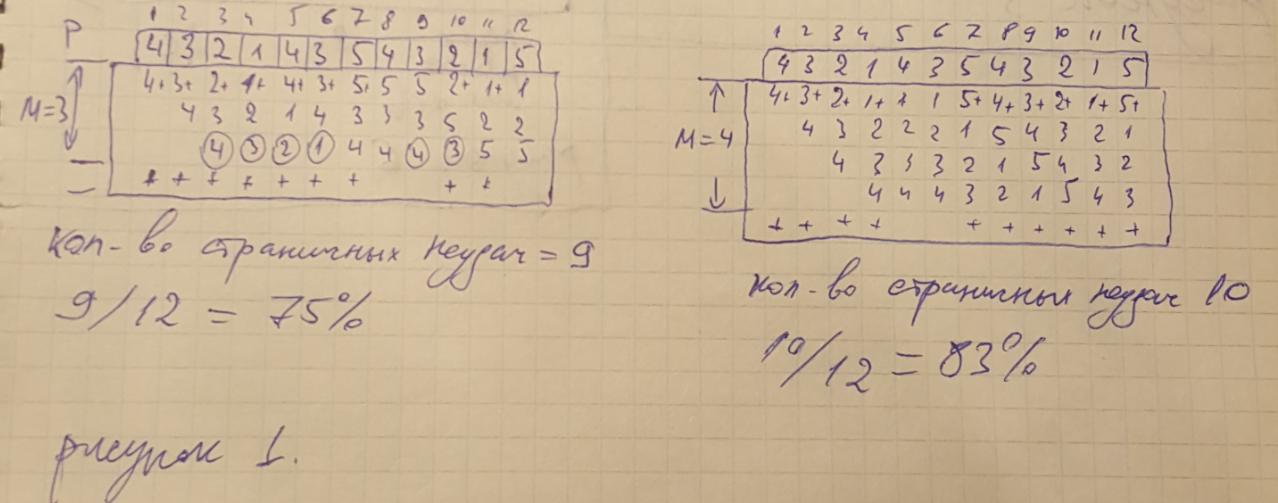
\includegraphics[width=\textwidth]{pic/8.png}
    \caption{pic}
\end{figure}

\subsubsection{LRU}

Может быть организован с помощью временных меток или связанного списка. При каждом обращении к странице временная метка обновляется. Если связный список, то страница переносится в хвост. Никогда не будет вытолкнута часто используемая страница. Но алгоритм требует больших накладных расходов. В основе этого алгоритма лежит эвристическое правило, что если обращение было к странице, то следующее обращение будет к этой же странице. Связано со свойством локальности, характерным для наших программ. Проведем моделирование на этой же модели.

\begin{figure}[H]
    \centering
    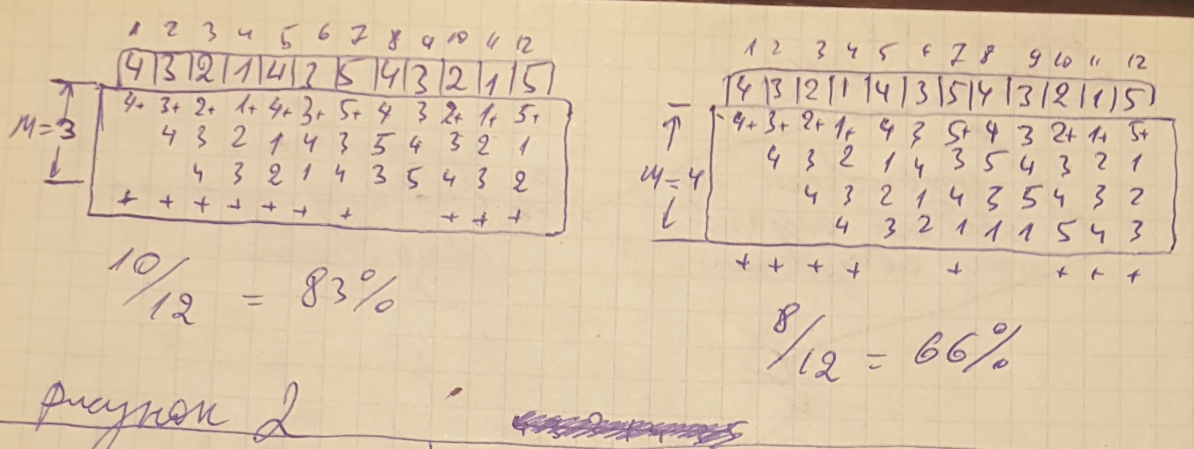
\includegraphics[width=\textwidth]{pic/9.png}
    \caption{pic}
\end{figure}

Свойство включения – первые три строки совпадают. Алгоритм относится к классу стековых алгоритмов. Никогда не приведет к росту числа страничных прерываний при увеличении памяти. Крайне затратный. Связан с постоянным редактированием. В чистом виде не используется. Используется аппроксимация LRU.

\subsubsection{Алгоритм NUR}

Cтраница не используемая в последнее время. 

\begin{figure}[H]
    \centering
    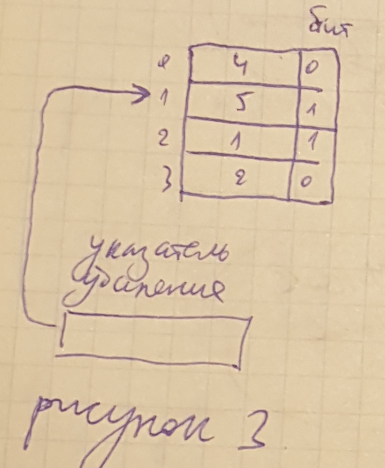
\includegraphics[width=\textwidth]{pic/10.png}
    \caption{pic}
\end{figure}

момент загрузки 5 страницы в первый кадр. Указатель удаления установлен на первый кадр. Если в дальнейшем потребуется удалить страницу, то проверку битов обращения будут начинать со второго кадра.
Каждой странице приписывается бит обращения. В какие то моменты времени все биты сбрасываются в ноль. Затем при обращении к странице бит обращения устанавливается в 1. Для вытеснения ищется первая страница, у которой бит обращения = 0. Есть бит обращения.  Так же важен бит модификация. Если модификации не было, то точная копия находится на диске и её не надо копировать (мы избавляемся от необходимости копирования). 

\begin{table}[H]
\begin{tabular}{|l|l|}
\hline
Бит обращения & Бит модификации\\
\hline
0 & 0 \\
\hline
0 & 1 \\
\hline
1 & 0 \\
\hline
1 & 1\\
\hline
\end{tabular}
\end{table}

Выгодно выгружать не модифицируемые страницы.

\subsubsection{LFU наименее часто используемая страница}

Эта стратегия близка к LRU. В ней контролируется частота обращения к странице. Может быть вытолкнута только что загруженная страница. 

\subsubsection{Метод связанных пар}

Эти рассуждения связанны с размером страницы. На конкретной странице выполняется только часть команд. Чем больше размер страницы, тем меньшее количество команд будет выполнено.  Если адресное пространство процесса поделено на небольшие страницы, то возрастает размер таблицы страниц. При это таблица страниц должна находиться в оперативной памяти. 

\begin{figure}[H]
    \centering
    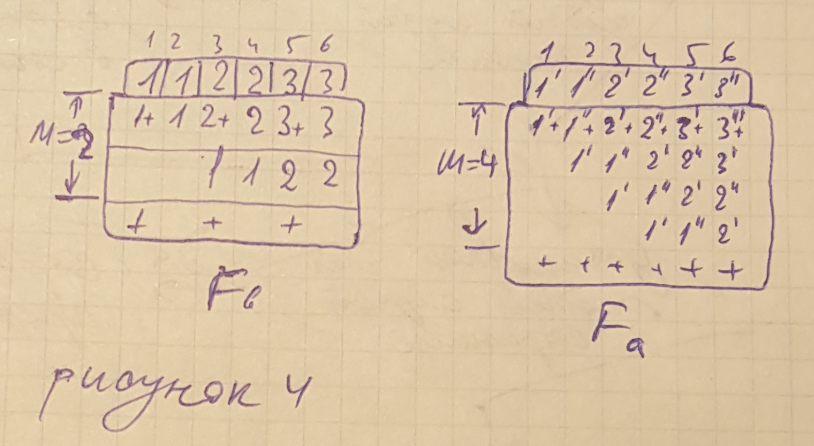
\includegraphics[width=\textwidth]{pic/11.png}
    \caption{pic}
\end{figure}

В 1973 году Медник показал, что для LRU существуют траектории страниц такого вида, для которых отношение числа страничных прерывания $Fa / Fb$ будет стремиться к $M/N + 1$, где $N$ - размер страницы. $1024 / 4  + 1 = 257$. 
Наиболее часто употребим размер страницы 4 кб.

\subsection{Вытеснения}

Глобальное вытеснение – вытеснение любой страницы любого процесса. Локальное вытеснение – страница для вытеснения выбирается из пула загруженных страниц данного процесса. 

\paragraph{Страничное поведение программ. Производительность.}

\begin{figure}[H]
    \centering
    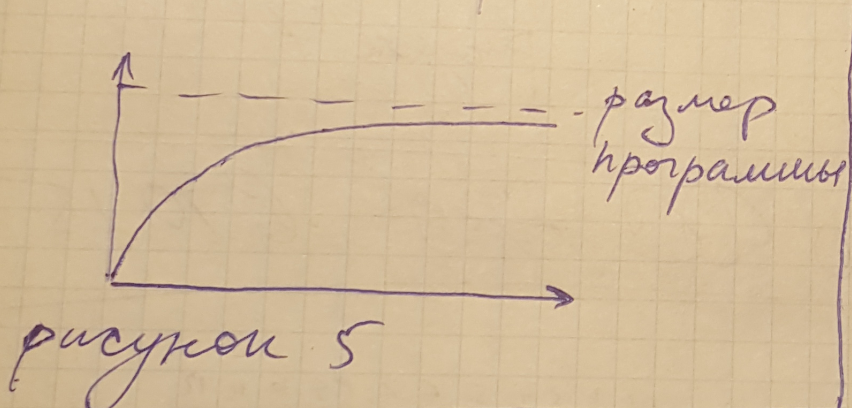
\includegraphics[width=\textwidth]{pic/12.png}
    \caption{График, который показывает процент страниц, к которым процесс обращается в течении своей жизни.}
\end{figure}

Минимально необходимая память: Страница кода (точка входа), страница сегмента данных, страница сегмента стека. Получив квант процессора, процесс начинает интенсивно подкачивать страницы. За время существования процесс обратится к большей части своих страниц. Этот перегиб связан с тем, что процесс для своего нормального выполнения, без страничных прерываний (увеличивают время выполнения процесса). Если процессу удается загрузить в память все страницы, к которым он обращается, то он будет выполняться без страничных прерываний. Этот факт получил название – теория рабочего множества. Поведение программы, во время выполнения, с точки зрения загрузки страниц, не является стабильным. Страничное поведение процесса не является стабильным. 
Деннинг 1968 году предложил в качестве локальной меры произвольности взять число страниц, к которым программа обращается за интервал времени $\Delta t$. $W(t, dt)$ – рабочее множество. Если процессу удается загрузить в память всё рабочее множество, то процесс будет выполняться без страничных прерываний, т.е. эффективно. Если процесс не сможет загрузить всё свое рабочее множество (страницы, которые ему необходимы в данный промежуток времени $\Delta t$), то возникнет подкачка одних и тех же страниц, названная \textbf{трешингом [thrashing]}.

\begin{figure}[H]
    \centering
    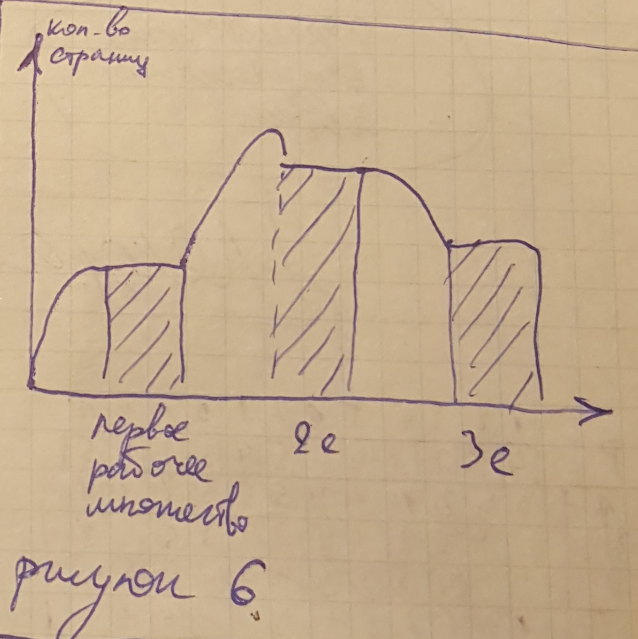
\includegraphics[width=\textwidth]{pic/13.png}
    \caption{pic}
\end{figure}

В процессе жизни процесса он обращается к разным набором страниц. Загрузив рабочее множество, процесс будет выполняться без страничных прерываний. Затем ему нужно перейти в другое рабочее множество.  
